% This file is part of TenSing-Moers/Theaterskript2018.
%
% TenSing-Moers/Theaterskript2018 is free content: you can redistribute and/or
% modify it under the terms of the cc-by-nc-sa (Creative Commons
% Attribution-NonCommercial-ShareAlike) as released by the
% Creative Commons organisation, version 4.0.
%
% TenSing-Moers/Theaterskript2018 is distributed in the hope that it will be useful,
% but without any warranty.
%
% You should have received a copy of the cc-by-nc-sa-license along
% with this copy of TenSing-Moers/Theaterkskript2018. If not, see
% <https://creativecommons.org/licenses/by-nc-sa/4.0/legalcode>.
%
% Copyright TenSing Moers and all whose work and <3 went in this project.
\documentclass[oneside,12pt,enabledeprecatedfontcommands]{scrartcl}
\usepackage[ngerman]{babel} %Deutsche Sprachunterstützung
\usepackage{scrpage2} %Kopf- und Fußzeilen
\usepackage[utf8]{inputenc} %Umlaute
%\usepackage{tabularx}
\usepackage{dramatist} %Dramatist-Package für minimale Charakterdefinitionen, Bühnenanweisungen, ... (dramatist.sty im Verzeichnis hinterlegen)
\usepackage[x11names]{xcolor} %Farben
\usepackage[skins]{tcolorbox} %Die für die Sprechakte verwendete Colorbox
\pagestyle{scrheadings}
\usepackage{tikz} %Grafiken, ursprünglich für cooleres "hervorheben". Jetzt zur Dekoration der Section Headings!
%\usetikzlibrary{decorations}
%\usepackage[bookmarks]{hyperref} %Verlinkungen im Inhaltsverzeichnis, um per Klicken zu den entsprechenden Szenen zu springen
%\usepackage[paper=a4paper,top=20mm,left=20mm,bottom=20mm,right=20mm,headheight=2cm,includehead,includefoot]{geometry} %Seitenrand einstellen
\usepackage[paper=a4paper,top=10mm,left=15mm,bottom=10mm,right=15mm,headheight=1cm,footskip=1cm,includefoot]{geometry} %Seitenrand einstellen
%\usepackage{xpatch} % disabled for debugging
%\usepackage{showframe} % Provides \xapptocmd % disabled for debugging
\usepackage{titlesec} %Dekoration der Section Headings, s. unten
\usepackage{setspace} %Zeilenabstand
\usepackage{soul} %Striketrough \st{}
%\usepackage{amsfonts} %\circledR-Kommando für registered trademark symbol % disabled for debugging
\usepackage{multicol}
%\usepackage[pages=some]{background} % disabled for debugging % INCOMPATIBLE TO ADVANCEDPERSONLISTS.TEX 2.0!!
\usepackage{eso-pic} % background % disabled for debugging

% Colorboxen für die hervorgehobenen Namen
\tcbset{commonstyle/.style={boxrule=0pt,sharp corners,enhanced jigsaw,hbox,nobeforeafter,boxsep=0pt,left=\fboxsep,right=\fboxsep}}
\newtcolorbox{mycolorbox}[1][]{commonstyle,#1}
\newlength\myboxwidth
\setlength{\myboxwidth}{\dimexpr\textwidth-2\fboxsep}

%\usepackage{soul}
\usepackage{tikz}
\usetikzlibrary{calc}
\usetikzlibrary{decorations.pathmorphing}

\makeatletter

\newcommand{\defhighlighter}[3][]{%
  \tikzset{every highlighter/.style={color=#2, fill opacity=#3, #1}}%
}

\defhighlighter{yellow}{.5}

\newcommand{\highlight@DoHighlight}{
  \fill [ decoration = {random steps, amplitude=1pt, segment length=15pt}
        , outer sep = -15pt, inner sep = 0pt, decorate
        , every highlighter, this highlighter ]
        ($(begin highlight)+(0,8pt)$) rectangle ($(end highlight)+(0,-3pt)$) ;
}

\newcommand{\highlight@BeginHighlight}{
  \coordinate (begin highlight) at (0,0) ;
}

\newcommand{\highlight@EndHighlight}{
  \coordinate (end highlight) at (0,0) ;
}

\newdimen\highlight@previous
\newdimen\highlight@current

\DeclareRobustCommand*\highlight[1][]{%
  \tikzset{this highlighter/.style={#1}}%
  \SOUL@setup
  %
  \def\SOUL@preamble{%
    \begin{tikzpicture}[overlay, remember picture]
      \highlight@BeginHighlight
      \highlight@EndHighlight
    \end{tikzpicture}%
  }%
  %
  \def\SOUL@postamble{%
    \begin{tikzpicture}[overlay, remember picture]
      \highlight@EndHighlight
      \highlight@DoHighlight
    \end{tikzpicture}%
  }%
  %
  \def\SOUL@everyhyphen{%
    \discretionary{%
      \SOUL@setkern\SOUL@hyphkern
      \SOUL@sethyphenchar
      \tikz[overlay, remember picture] \highlight@EndHighlight ;%
    }{%
    }{%
      \SOUL@setkern\SOUL@charkern
    }%
  }%
  %
  \def\SOUL@everyexhyphen##1{%
    \SOUL@setkern\SOUL@hyphkern
    \hbox{##1}%
    \discretionary{%
      \tikz[overlay, remember picture] \highlight@EndHighlight ;%
    }{%
    }{%
      \SOUL@setkern\SOUL@charkern
    }%
  }%
  %
  \def\SOUL@everysyllable{%
    \begin{tikzpicture}[overlay, remember picture]
      \path let \p0 = (begin highlight), \p1 = (0,0) in \pgfextra
        \global\highlight@previous=\y0
        \global\highlight@current =\y1
      \endpgfextra (0,0) ;
      \ifdim\highlight@current < \highlight@previous
        \highlight@DoHighlight
        \highlight@BeginHighlight
      \fi
    \end{tikzpicture}%
    \the\SOUL@syllable
    \tikz[overlay, remember picture] \highlight@EndHighlight ;%
  }%
  \SOUL@
}
\makeatother

%Deckblatt
%\title{Die Drei Anführungszeichen und schon wieder irgendwas}
%\author{(Working Title)\\TenSing Moers 2016}
%\date{2016}

\newcommand{\myquote}[1]{\glqq #1\grqq}

\setlength{\parskip}{0mm} %3mm Abstand nach jedem Absatz
\setlength{\parindent}{0pt} %Dummes Absatz-Eingerücke abstellen
\newlength{\dramatextinset}
\setlength{\dramatextinset}{\dimexpr-\leftmargin+\labelsep}
\edef\savedfboxsep{\the\fboxsep} %Speichere den fboxsep, da dieser später (lied, tanz, etc.-commands) verändert wird, und offenbar nicht zurückgestellt wird. Dies verursacht Probleme mit den Hervorhebungen der Charakternamen, da das Margin der Highlight-Colorboxen nach einem Aufruf von \lied sehr gering ist.

% Disabled for debugging
%\xapptocmd{\drama}{%
%\setlength{\parindent}{\dramatextinset}%
%}{\typeout{Success}}{\typeout{Failure}}

%Übersetzung der standartmäßig englischen Namen "Characters", "Act", "Scene" ins Deutsche
\renewcommand{\casttitlename}{Personen}
\renewcommand{\actname}{Akt}
\renewcommand{\scenename}{Szene}
\renewcommand{\casttitlefont}{\scshape \bf \LARGE}
\renewcommand{\scenenamefont}{\scshape \LARGE}
%Ursprüngliche Anpassung des Szenennamens:
%\renewcommand{\printscenename}{\clearpage\centering\scenenamefont \scenename} %Die Aktnummer soll nicht abgedruckt werden, da dies ein "Einakter" ist.

%Anpassung des Szenennamens im "coolen Design":
\renewcommand{\thescene}{\Roman{scene}} %Anpassung der Szenenummern in große statt kleine römische Zahlen
%Dieses Kommando hinterlegt den aktuellen Text in der gesamten Breite mit einer orangenen Box
\newcommand{\sechl}{\tikz[overlay]{ \draw[fill=OliveDrab2] (-.6\textwidth,-1ex) rectangle (1.15\textwidth,1em);}}%\draw (-.75\textwidth,-1ex) -- (\textwidth,-1ex); \draw (-\textwidth,1em) -- (\textwidth,1em)}%}
\newcommand{\sechlg}{\tikz[overlay]{ \draw[fill=Turquoise2] (-.6\textwidth,-1ex) rectangle (1.15\textwidth,1em);}}%\draw (-.75\textwidth,-1ex) -- (\textwidth,-1ex); \draw (-\textwidth,1em) -- (\textwidth,1em)}%}
\renewcommand{\printscenename}{\vspace{2cm}\huge\bfseries\center\sechl \scenename}
%\renewcommand{\printscenename}{\clearpage\huge\bfseries\center\sechl \scenename} %Die Aktnummer soll nicht abgedruckt werden, da dies ein "Einakter" ist.
\renewcommand{\printscenenum}{\stepcounter{section}\scenenumfont \thescene} %Die Kapitelnummer soll bei jeder neuen Szene hochgezählt werden, damit Unterteilungen mit entsprechenden Nummern möglich sind
\renewcommand{\printscenetitle}[1]{\scenetitlefont: #1}

%Dekoration der Section Headings
\titleformat{\section}[block]% Abgewandelt nach http://tex.stackexchange.com/questions/104336/fancy-heading-section-titles-disappears
 {\clearpage\huge\bfseries\center\sechl}
 {\thesection}%
 {1em}%
 {}

%Dekoration der Subsection-Headings
\titleformat{\subsection}[block]% Abgewandelt nach http://tex.stackexchange.com/questions/104336/fancy-heading-section-titles-disappears
 {\huge\bfseries\center\sechlg}
 {\thesubsection}%
 {1em}%
 {}

%\StageDirConf{\setlength{\parindent}{0pt}\par\itshape}{}
%\StageDirConf{\setlength{\parskip}{3mm}\vspace{-1mm}\begin{quote}}{\end{quote}\vspace{-1mm}}

%Ein Kommando, welches in blauer Farbe und in Klammern und Kursiv die Besetzung jeder Rolle in den DramaticsPersonae abdruckt (wird dort verwendet)
\newcommand{\role}[1]{\textcolor{blue}{(\textit{#1})}}

%\newcommand\hl[2]{\tikz[baseline,decoration={random steps,amplitude=1pt,segment length=15pt},outer sep=-15pt, inner sep = 0pt]\node[decorate,rectangle,fill=#1,anchor=text]{#2\xspace};}

%Kommandos für die Infos vor jeder Szene (Requisiten, Spielort, Charaktere)
\newcommand{\ort}[1]{\textbf{Ort:} \textit{#1}\par}
\newcommand{\requ}[1]{\textbf{Requisiten:} \textit{#1}\par}
\newcommand{\chars}[1]{\begin{spacing}{1.5}\textbf{Charaktere:} \textit{#1}\end{spacing}\par}

% Kommandos, um die Sprechtexte der Charactere darzustellen
\newcommand{\speechbox}[4]{\item\leavevmode\begin{tcolorbox}[before={},after={},title=#1,colframe=#2,coltitle=#3]#4\end{tcolorbox}}
%\newcommand{\speechbox}[3]{\item\leavevmode\begin{tcolorbox}[before={},after={},title=#1,colframe=#2]#3\end{tcolorbox}}
%\newcommand{\speechboxblack}[3]{\item\leavevmode\begin{tcolorbox}[before={},after={},title=#1,colframe=#2,coltitle=black]#3\end{tcolorbox}}
%\newcommand{\speechbox}[3]{\item\leavevmode\begin{tcolorbox}[before={\hskip\dimexpr\leftmargin-\speechskip},after={},title=#1,colframe=#2]#3\end{tcolorbox}}
%\newcommand{\speechbox}[3]{\item\leavevmode\mbox{}\begin{tcolorbox}[before={\hskip\dimexpr\leftmargin-\speechskip},after={},title=#1,colframe=#2]#3\end{tcolorbox}}

\newcommand{\delim}{, } %Der Zeilentrenner in den Charakterlisten

\newcommand{\sep}{\\[3mm]} %Um einen Zeilenumbruch mit Abstand ("fake-Absatz") innerhalb der tcolorboxen zu erzeugen

%Kommandos, um die Programmpunkte im Skript zu vermerken
%\newcommand{\lied}[1]{\colorbox{DarkOliveGreen2}{\parbox{\textwidth}{\textbf{Lied: } #1}}}
\newcommand{\lied}[2]{\fboxsep0mm\colorbox{DarkOliveGreen2}{\fboxsep4mm\framebox[\textwidth][l]{\parbox{\linewidth}{\Large\textbf{\textsc{Lied}: } #1 $\Biggl\vert$ \textsubscript{#2}}}}}
\newcommand{\tanz}[1]{\fboxsep0mm\colorbox{SteelBlue1}{\fboxsep4mm\framebox[\textwidth][l]{\parbox{\linewidth}{\Large\textbf{\textsc{Tanz}: } #1}}}}
\newcommand{\pause}{\fboxsep0mm\colorbox{SteelBlue1}{\fboxsep4mm\framebox[\textwidth][l]{\parbox{\linewidth}{\center\Huge\textsc\textbf{\textsc{--------- Pause! ---------}}}}}}
\newcommand{\other}[1]{\fboxsep0mm\colorbox{SteelBlue1}{\fboxsep4mm\framebox[\textwidth][l]{\parbox{\linewidth}{\center\huge\textsc\textbf{#1}}}}}
\newcommand{\boxcommand}[2]{\setlength{\fboxsep}{\savedfboxsep}\colorbox{#1}{#2}} %Dieses Kommando bestimmt, wie jedes der Highlight-Makros seine Colorboxen macht. Die Länge \fboxsep muss jedes mal neu gesetzt werden, da die colorboxen in \lied, \tanz usw, diese auf 0mm setzen, und nicht wieder zurücksetzen. Sonst sieht der Margin trotz \strut hässlich aus.
\newcommand{\mikroan}[1]{\fboxsep0mm\colorbox{Orange1}{\fboxsep2mm\framebox[0.3\textwidth][l]{\parbox{\linewidth}{\vspace{0mm}\textsc\textbf{Mikro an: #1}}}}}
\newcommand{\mikroaus}[1]{\par\fboxsep0mm\colorbox{Orange1}{\fboxsep2mm\framebox[0.3\textwidth][l]{\parbox{\linewidth}{\vspace{0mm}\textsc\textbf{Mikro aus: #1}}}}}
\newcommand{\sound}[1]{\begin{flushright}
\par\fboxsep0mm\colorbox{Green2}{\fboxsep2mm\framebox[0.3\textwidth][l]{\parbox{\linewidth}{\vspace{0mm}\textsc\textbf{Sound: #1}}}}
\end{flushright}}
\newcommand{\soundwide}[1]{\begin{flushright}
\par\fboxsep0mm\colorbox{Green2}{\fboxsep2mm\framebox[0.5\textwidth][l]{\parbox{\linewidth}{\vspace{0mm}\textsc\textbf{Sound: #1}}}}
\end{flushright}}

% disabled for debugging
%\backgroundsetup{
%scale=1,
%color=black,
%opacity=0.4,
%angle=0,
%contents={%
%  \includegraphics[width=\paperwidth, height=\paperheight]{example-image}
%  }%
%}

\newcommand\BackgroundPic{%
\put(0,0){%
\parbox[b][\paperheight]{\paperwidth}{%
\vfill
\centering
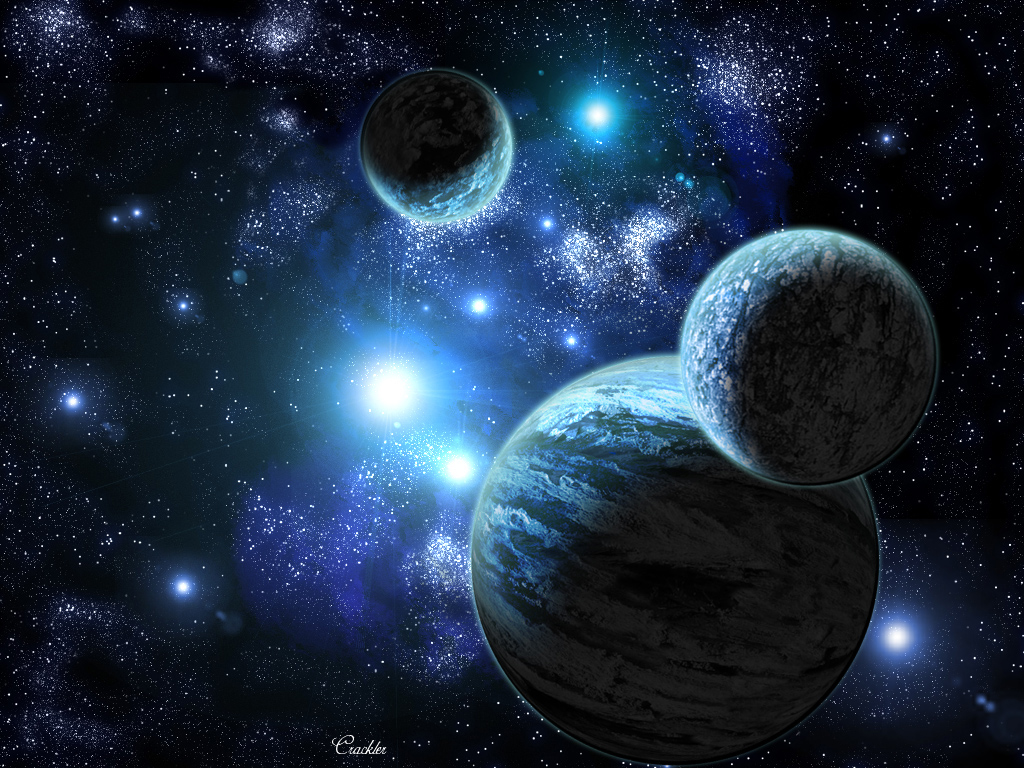
\includegraphics[%width=\paperwidth,
height=\paperheight,keepaspectratio]{res/Space-2.jpg}%
\vfill
}}}